\documentclass[12pt]{article}

\usepackage{answers}
\usepackage{setspace}
\usepackage{graphicx}
\usepackage{enumitem}
\usepackage{multicol}
\usepackage{mathrsfs}
\usepackage[margin=1in]{geometry} 
\usepackage{amsmath,amsthm,amssymb,mathtools}
\usepackage{titlesec}

\newcommand\numberthis{\addtocounter{equation}{1}\tag{\theequation}}

\titleformat{\section}[runin]{\normalfont\Large\bfseries}{\thesection}{1em}{}
\titleformat{\subsection}[runin]{\normalfont\large\bfseries}{\thesubsection}{1em}{}

\def\tf{\textbf}
\def\tt{\textit}
\def\mc{\ensuremath\mathcal}
\def\mf{\ensuremath\mathbf}
\def\mt{\ensuremath\mathit}
\def\mb{\ensuremath\mathbb}
\def\td{\ensuremath\tilde}
\def\N{\ensuremath\mb{N}}
\def\Z{\ensuremath\mb{Z}}
\def\C{\ensuremath\mb{C}}
\def\R{\ensuremath\mb{R}}
\def\S{\ensuremath\mb{S}}
\def\Ber{\ensuremath\mf{Ber}}
\def\det{\ensuremath\mf{det}}
\def\sigm{\ensuremath\mf{sigm}}
\def\diag{\ensuremath\mf{diag}}
\def\dom{\ensuremath\mf{dom}}
\def\cond{\ensuremath\mf{cond}}
\def\sign{\ensuremath\mf{sign}}
\def\bd{\ensuremath\mf{bd}}
\def\rto{\ensuremath\rightarrow\ }
\def\Rto{\ensuremath\Rightarrow\ }
\def\lto{\ensuremath\leftarrow\ }
\def\Lto{\ensuremath\Leftarrow\ }
\def\xrto{\ensuremath\xrightarrow}
\def\xRto{\ensuremath\xRightarrow}
\def\xlto{\ensuremath\xleftarrow}
\def\xLto{\ensuremath\xLeftarrow}
\def\rvec{\ensuremath\overrightarrow}
\def\lvec{\ensuremath\overleftarrow}

\providecommand\P[1]{}
\renewcommand\P[1]{\mb{P}\{#1\}}
\providecommand\E[1]{}
\renewcommand\E[1]{\mb{E}[#1]}
\providecommand\Var[1]{}
\renewcommand\Var[1]{\mf{Var}(#1)}
\providecommand\p[2]{}
\renewcommand\p[2]{\frac{\partial #1}{\partial #2}}
\providecommand\pp[2]{}
\renewcommand\pp[2]{\frac{\partial^2 #1}{\partial #2^2}}
\providecommand\ps[3]{}
\renewcommand\ps[3]{\frac{\partial^2 #1}{\partial #2\partial #3}}
\providecommand\d[2]{}
\renewcommand\d[2]{\frac{d #1}{d #2}}

\DeclareMathOperator{\sech}{sech}
\DeclareMathOperator{\csch}{csch}
    
\begin{document}
    
\title{Complex Integration: Cauchy's Theorem - Notes}
\author{Dhruv Kohli}
\maketitle
\section{Introduction}
\begin{itemize}
    \item $\int_{a}^{b}$ in $\R$ has only way to from $a$ to $b$ but in $\C$, the two points are in a plane. In general, the integral will depend on the path (countour) taken.
    \item Unlike differentiation which made sense for strictly limited set of analytic functions, integration of non-analytic function is possible.
    \item We will see under what conditions the value of integral is independent of contour.
    \item Cauchy's Theorem essentially says that any two integrals from $a$ to $b$ will agree, provided that the mapping is \tt{analytic everywhere in the region lying between the two countours}.
\end{itemize}
\section{The Real Integral}
\begin{itemize}
    \item \tt{Riemann sum} $R \equiv \sum_{i=1}^{n}f(x_i)\Delta_i$. Desired area can be obtained by simultaneously letting $n$ tend to $\infty$ while each $\Delta_i$ shrinks to nothing. There are many ordinary functions whose antiderivative does not exist. That's when we will require Riemann sum.
    \item Two familiar ways to compute $R$ are trapezoidal rule and Simpson's rule.
    \item The trapezoid rule can be accurately approximated by Riemann sum using a modest value of $n$ and choosing $x_i$ to be the midpoint of its $\Delta_i$. This is called \tt{Midpoint Riemann Sum} $R_M$.
\end{itemize}
\section{The Complex Integral}
\subsection{Complex Riemann Sums}
\begin{figure}[h!]
    \centering
    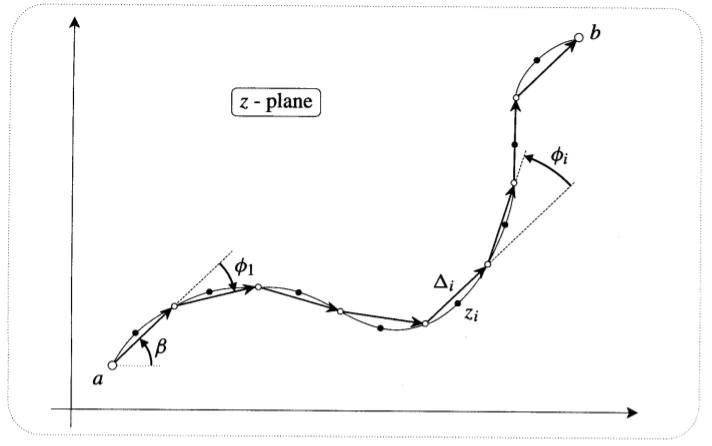
\includegraphics[scale=0.7]{fig_1}
    \label{f1}
\end{figure}
\begin{figure}[h!]
    \centering
    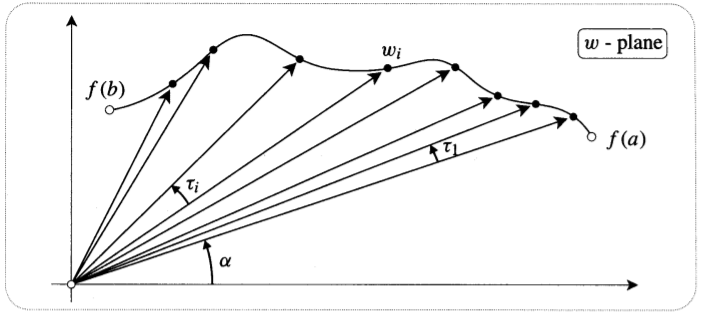
\includegraphics[scale=0.7]{fig_2}
    \label{f2}
\end{figure}
\begin{figure}[h!]
    \centering
    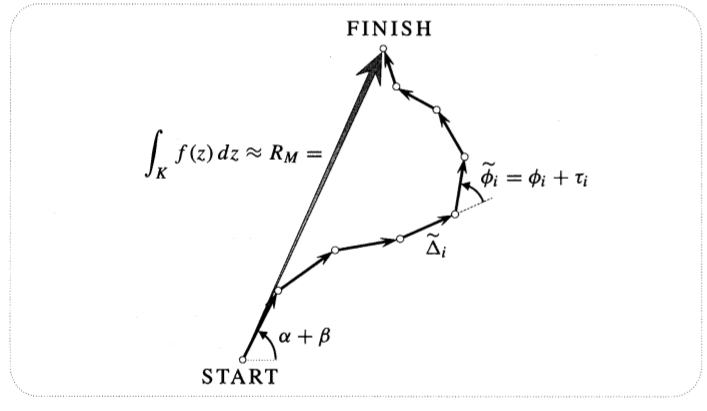
\includegraphics[scale=0.7]{fig_3}
    \label{f3}
\end{figure}
\subsection{A Useful Inequality}
\begin{itemize}
    \item If all $\Delta_i$ points in same direction then length of straightened version would just be sum of $|\td{\Delta}_i|$.
    \begin{align*}
        |R_M| &\leq \sum |w_i|\cdot |\Delta_i|
    \end{align*}
    with equality if and only if $\td{\phi}_i=0$. If $M$ denotes the maximum distance from the origin to the image curve,
    \begin{align*}
        |R_M| &\leq M \sum |\Delta_i|
    \end{align*}
    The summation term is the length of the polygonal approximation of $K$, so it cannot be greater than the actual length of $K$. So,
    \begin{align*}
        |\int_{K}f(z)dz| &\leq M \cdot (\text{length of }K)
    \end{align*}
    For example if $f(z)=(1/\bar{z})^2$ and $K$ is the circle $|z|=r$ then, $|\int_{K}f(z)dz| \leq (1/r)^22\pi r = 2\pi/r^2$. So as $r$ tends to $\infty$, $I\rto 0$.
\end{itemize}
\subsection{Rules of Integration}
\begin{align*}
    \int_{K}c f(z) dz &= c \int_{K}f(z)dz\\
    \int_{K}[f(z)+g(z)]dz &= \int_{K}f(z)dz + \int_{K}g(z)dz\\
    \int_{K+L}f(z)dz &= \int_{K}f(z)dz + \int_{L}f(z)dz (L\text{ begins at the end of }K)\\
    \int_{-K}f(z)dz &= -\int_{K}f(z)dz
\end{align*}
\begin{itemize}
    \item Note that the contour $K$ can have a kink. It shouldn't have infinitely many kinks.
    \begin{figure}[h!]
        \centering
        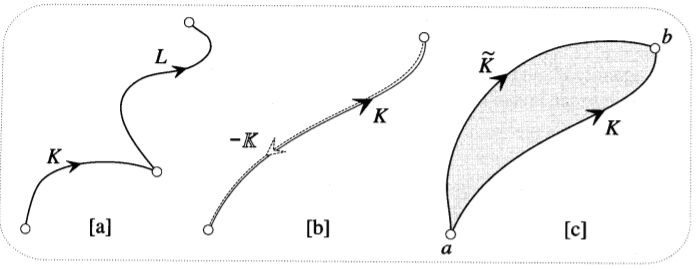
\includegraphics[scale=0.7]{fig_4}
        \label{f4}
    \end{figure}
    \item If two paths yield same integral then,
    \begin{align*}
        0 &= \int_{K}f(z)dz-\int_{\td{K}}f(z)dz\\
        &= \int_{K}f(z)dz + \int_{-\td{K}}f(z)dz\\
        &= \int_{K-\td{K}}f(z)dz
    \end{align*}
    \item If the integral vanishes for all closed loops through $a$ and $b$ then all curves between $a$ and $b$ will yield the same value for the integral. \tt{Path independence is equivalent to vanishing loop integrals}. The centerpiece of complex analysis is the link between this phenomenon and analyticity.
    \item Cauchy's Theorem consists in recognizing that the vanishing of loop integrals is the nonlocal manifestation of a local property of the mapping, namely, that it is an amplitwist everywhere inside the loop.
\end{itemize}
\section{Complex Inversion}
\subsection{A Circular Arc}
\begin{figure}[h!]
    \centering
    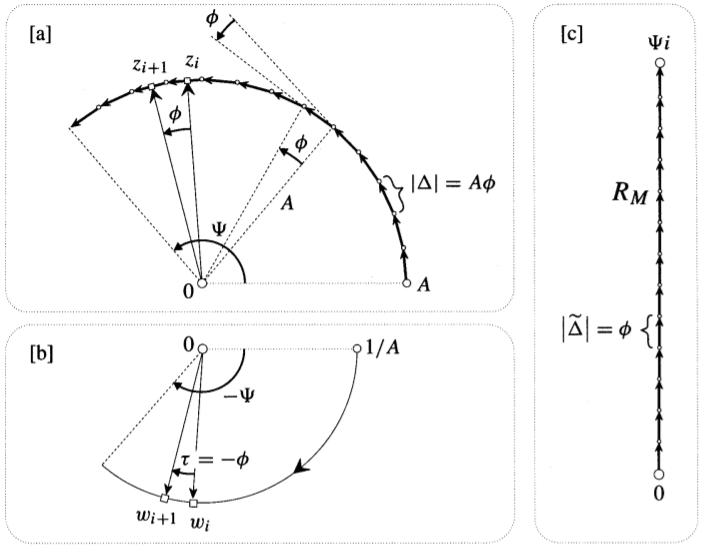
\includegraphics[scale=0.7]{fig_5}
    \label{f5}
\end{figure}
\begin{itemize}
    \item The value of $\int_{K}(1/z)dz$ where $K$ is an origin centered circle is $2\pi i$ (or for circular arc subtending angle $\Psi$ at center, $I=i\Psi$).
    \item This does not contradict with Cauchy's Theorem (which says that loop integrals vanish for analytic functions) because the theorem requires the function to be analytic \tt{everywhere} inside the loop. But our loops encloses origin at which analyticity of complex inversion breaks down.
\end{itemize}
\subsection{General Loops}
\subsection{Winding numbers}
\begin{itemize}
    \item If $L$ is any closed loop, then,
    \begin{align*}
        \oint_{L}(1/z)dz &= 2\pi i \nu(L,0)\\
        \oint_{L}(1/(z-p)) &= 2\pi i \nu(L,p)
    \end{align*}
\end{itemize}
\section{Conjugation}
\begin{itemize}
    \item Integration makes sense for any continuous complex mapping, regardless of whether it is anlaytic of not.
    \item But Cauchy's Theorem has no jurisdiction over non-analytic functions.
\end{itemize}
\end{document}
        